\cleardoublepage
\chapter*{Introduction}
\markboth{Introduction}{Introduction}
\addcontentsline{toc}{chapter}{Introduction}
% Here I bring the reader to general material science background to ML
% applications and their general importance, as well as the the study of
% representations as they are an essential building block

The discovery of new materials is one of the core pillars of technology, as
every technology relies on a material and, needless to say, would not exist
without it\cite{tomellini2013commentary}.
%[R. Tomellini, J. V. Benesch and A. Alming, Commentary: Fostering innovation
%in materials science and engineer].  A material can be more formally described
%by the configurations of atoms and the electron distribution.
The search for new materials is bound by thermodynamic laws which tell what
configurations are stable and can therefore be considered as potential
material.
%, i.e. can exist for a limited time frame under a certain set of thermodynamic
%boundary conditions.
In the last decades it has been shown that \textit{ab initio} quantum chemistry
methods provide approximate stability criteria which are in good agreement with
experiments\cite{jansen2015conceptual} making them a viable tool for the
screening of new materials\cite{ceder1998identification, andersson2006toward,
yang2012search, gomez2016design}.  Due to the vast number of possible atomic
structures to be considered, the efficiency of these methods is crucial.

Data-driven methods have become an efficient extension reducing expensive
quantum chemistry calculations to a bare minimum while reaching
close-to-\textit{ab initio} accuracy over a wide configuration
space\cite{bartok2018machine}, leading to the exploration of previously
computationally intractable problems, such as the thermal conductivity of
amorphous germanium telluride\cite{sosso2012thermal}.  These methods are based
on transforming geometrical, physical and chemical information into a vector
representation, referred as descriptor, to then use it as features in a machine
learning model.  The development of expressive and computational inexpensive
descriptors\cite{behler2011atom, bartok2013representing} has lead to
applications in a wide range of areas\cite{mansouri2018machine,
sosso2018understanding, basdogan2019machine}.  Efficient descriptors are
therefore essential for state of the art high-throughput material design
application.

%The key conceptual/domain part behind the methods determining their quality is
%the choice of description of the configuration called descriptor and the way
%to express similarity between these descriptions.

%0.5 page Statement of the problem and specific problem:
The efficient computation of expressive descriptors is a challenging problem
which has seen a wide range of proposals\cite{behler2011atom, rupp2012fast,
bartok2013representing, huo2017unified}.  It has been shown that
density-based state-of-the-art descriptors can be seen as different
representations of the symmetrized many-body correlation
function\cite{willatt2019atom}.
%The continuation of this development is the objective of this thesis.  The
%general goal of the thesis is the improvement of state of the art descriptors
%in terms of their encoded information and their concrete implementations.
Since machine learning models are based on comparing features with the help of
a similarity measurement, there is a strong connection between the similarity
of two atomic configurations in form of their descriptor, and the Euclidean
distance between their symmetrized many-body correlation function.
%The general goal of the thesis is the improvement of state of the art
%descriptors in terms of their encoded information and their concrete
%implementations.
While the Euclidean distance can represent distances between close
distributions accurately, more distant ones are not faithfully represented.  On
the other hand descriptors relying on sorting geometric
information\cite{rupp2012fast, gallet2013structural} are similarly connected to
the Wasserstein distance\cite{rowland2019orthogonal}.  The effect of the
distance among atomic environments on the descriptor and subsequently on the
regression of physical properties has not been extensively analyzed yet and is
part of the objective of this thesis.  Such an analysis requires the
development of measures for the comparison of feature spaces and efficient
adaptations of the Wasserstein distance to a wider range of descriptors.

Furthermore, recently generative models have been introduced for the generation
of stable atomic configurations\cite{Sanchez-Lengeling360, gebauer2019symmetry,
noe2019boltzmann, hoffmann2019data}.  The usage of descriptors in generative
models requires a mapping of the descriptor back to the atomic configuration.
Heretofore efficient inversion schemes have been introduced only for the
3-dimensional atomic density function\cite{Sanchez-Lengeling360} and for
distributions over distances between atoms\cite{gebauer2019symmetry}.  The
development of an efficient inversion for state of the art descriptors which
capture translational and rotational invariant many-body order information is
an open problem which will be addressed with this thesis.


\begin{figure}
    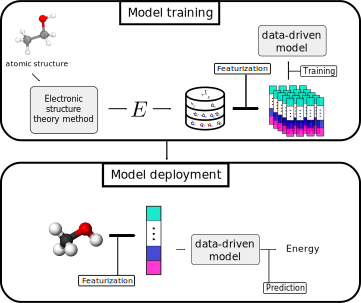
\includegraphics[width=\textwidth]{fig/slide5_0.png}
    \caption{High-throughput idea}
    \label{fig:high-throughput-scheme}
\end{figure}

